\documentclass{zjusct-beamer/zjusct}

% Metadata
\title{A First Look at the CPU Parallel Programming Framework} 
\subtitle{OpenMP \& MPI}
\author[YooLc]{Chenxiao Li (@YooLc)}
\date{\today}
\institute[ZJUSCT]{Zhejiang University Supercomputing Team}
\copyleftnotice{CC-BY 4.0}

\hypersetup{
    pdftitle={\title},
    pdfpagemode=FullScreen,
}

\begin{document}

% Set Mono and Emoji font
\setmonofont{DejaVu Sans Mono}
\setemojifont{TwemojiMozilla}

\maketitle

% Outline (Table of Contents)
\cutoc

\section{MPI}

\begin{frame}{History}
    \begin{columns}
    
        \begin{column}{0.55\textwidth}

    \begin{itemize}
        \item \textbf{Before 1990's}: Many libraries. 

        Writing code was a \alert{\textbf{difficult}} task.

        \vspace{0.2cm}
        \hrule{}
        \vspace{0.2cm}
        {\textbf{Models commonly adopted: Message Passing Model}}
        
        An application \alert{\textbf{passes messages}} among processes in order to perform a task.

        e.g. Job assignment, Results of sub-problems...
        
    \end{itemize}
    \end{column}

        \begin{column}{0.45\textwidth}
            \begin{itemize}
                \item Supercomputing '92

                Defined a \alert{\textbf{standard interface}}

                \item 1994

                MPI-1

                \item 2025.6.5
            
                MPI-5.0 Standard Release
            \end{itemize}
        \end{column}
    \end{columns}
    %\footnotetext{https://mpitutorial.com/tutorials/mpi-introduction/}

    %\footnotetext{https://www.mpi-forum.org/docs/}
\end{frame}

\begin{frame}{What is MPI}
    MPI, a \alert{\textbf{M}}essage \alert{\textbf{P}}assaing \alert{\textbf{I}}nterface.

    There exists many implementations:
    \begin{itemize}
        \item OpenMPI
        \item Intel-MPI
        \item MPICH
        \item HMPI (Hyper-MPI)
        \item ......
    \end{itemize}

    \textbf{Kindly Reminder}: Please do not mess up MPI implementations with MPI standard.
\end{frame}


\begin{frame}{Installation}
    \begin{itemize}
        \item OpenMPI
        
            Lab0
        \item Intel-MPI: Included in \href{https://www.intel.cn/content/www/cn/zh/developer/tools/oneapi/toolkits.html}{Intel- neAPI}
        
            Can be installed using spack

        \item HMPI: \href{https://support.huawei.com/enterprise/zh/doc/EDOC1100228708/c5d7ef16}{Huawei}
    \end{itemize}
\end{frame}

\begin{frame}[fragile]{Hello MPI World!}
    \begin{minted}[fontsize=\scriptsize]{c}
#include <mpi.h>
#include <stdio.h>
int main(int argc, char** argv) {
    MPI_Init(&argc, &argv);
    int world_size;
    MPI_Comm_size(MPI_COMM_WORLD, &world_size);
    int world_rank;
    MPI_Comm_rank(MPI_COMM_WORLD, &world_rank);
    char processor_name[MPI_MAX_PROCESSOR_NAME];
    int name_len;
    MPI_Get_processor_name(processor_name, &name_len);
    printf("Hello world from processor %s, rank %d out of %d processors\n",
    processor_name, world_rank, world_size);
    MPI_Finalize();
    return 0;
}
    \end{minted}
\end{frame}

\subsection{Basic Concepts}

\begin{frame}{Communicator}
    \begin{block}{Definition}
        A communicator defines a group of processes that have the ability to communicate with one another.
        
        Each process has a \alert{\textbf{unique rank}}.
    \end{block}
\end{frame}


\begin{frame}{Communicator (cont.)}
\begin{columns}
    \begin{column}{.6\textwidth}
        \begin{itemize}
        \item MPI\_COMM\_WORLD
        \end{itemize}
        \begin{figure}
            \centering
            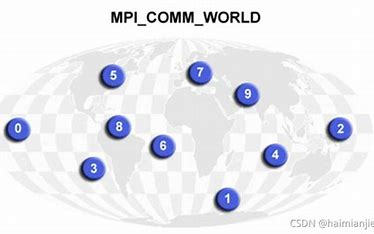
\includegraphics[width=\linewidth]{day8_am/img/mpi/mpi_comm_world.png}
            \caption{}
            \label{fig:mpi_comm_world}
        \end{figure}
    \end{column}
\end{columns}

\end{frame}


\begin{frame}{Communicator (cont.)}
\begin{columns}
    \begin{column}{.6\textwidth}
    \begin{itemize}
        \item MPI\_COMM\_SPLIT

        \begin{itemize}
            \item comm: The communicator that will be used as the basis for the new communicators.
            \item color: Which new communicator each processes will belong.
            \item key: The ordering (rank) within each new communicator.
            \item new\_comm: [OUT]
        \end{itemize}
    \end{itemize}
    \end{column}
        \begin{column}{.4\textwidth}
        \begin{figure}
            \centering
            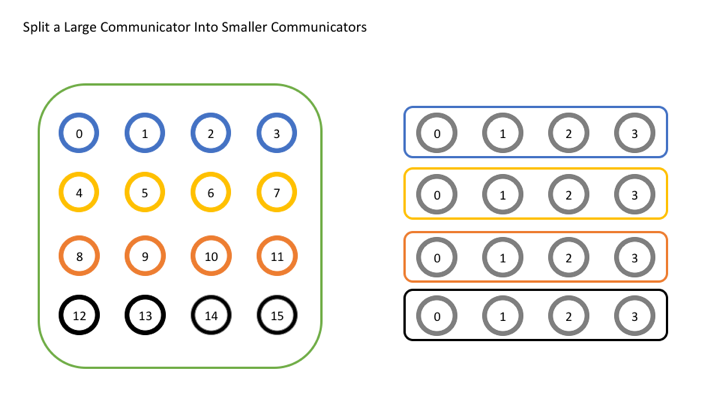
\includegraphics[width=1.0\linewidth]{day8_am/img/mpi/commsplit.png}
        \end{figure}
    \end{column}
\end{columns}

\end{frame}

\begin{frame}{Blocking vs Non-blocking}
    \begin{columns}
        \begin{column}{.5\textwidth}
            \textbf{\large Blocking}

            It does not return until the message data and envelope have been \alert{\textbf{safely stored away}} so that the sender is free to modify the send buffer. 
            
            The message might be copied directly into the \alert{\textbf{matching receive buffer}}, or it might be copied into a \alert{\textbf{temporary system buffer}}.
        \end{column}
        \begin{column}{.5\textwidth}
            \textbf{\large Non-blocking}

            A nonblocking call initiates the operation, but does not complete it. 
            
            They will return \alert{\textbf{almost immediately}}.
            
        \end{column}
    \end{columns}
\end{frame}

\begin{frame}{Order}
    \textbf{\large Messages are non-overtaking}
    
    Order is preserved.(Only under single thread)

If a sender sends two messages in succession to the same destination, and both match the same receive, then this operation cannot receive the second message if the first one is still pending. 

If a receiver posts two receives in succession, and both match the same message, then the second receive operation cannot be satisfied by this message, if the first one is still pending.
\end{frame}

\begin{frame}{Fairness}
    MPI makes \alert{\textbf{no guarantee}} of fairness in the handling of communication.

    There may be starvation.

    \begin{example}
        Rank1 $\rightarrow ^{send}$ Rank0

        Rank2 $\rightarrow^{send}$ Rank0

        Rank0 $\leftarrow^{receive}$ from any source.
    \end{example}
\end{frame}
\subsection{OpenMP directives and constructs}

\begin{frame}[fragile]{OpenMP Directives}

  \begin{block}{A legal OpenMP Directive must has the following format (C/C++):}
    \begin{tabular}{|c|c|c|c|}
      \hline
      Pragma       & Directive                       & [clause[ [,]clause] ... ] \\
      \hline
      \#pragma omp & parallel, atomic, critical, ... & 0 to many                 \\
      \hline
    \end{tabular}
  \end{block}
  \begin{itemize}
    \item \emoji{chestnut} \textbf{For example:}
          \vspace{-5pt}
          \begin{minted}[fontsize=\scriptsize]{c}
#pragma omp parallel for collapse(2) private(tmp_v, d, v)
    \end{minted}
    \item Case sensitive
    \item Affects the block (single statement or wrapped by \verb|{}|) after this directive
    \item \emoji{zany-face} Here's an official \href{https://www.openmp.org/wp-content/uploads/OpenMPRefCard-5-2-web.pdf}{\textbf{Cheet Sheet}}
  \end{itemize}
\end{frame}

\begin{frame}[fragile]{Constructs}
  \emoji{thinking} What is the difference between \textbf{construct} and \textbf{directive}?

  \emoji{nerd-face} An OpenMP construct is a formation for which the directive is executable.\footnote{https://www.openmp.org/spec-html/5.2/openmpse14.html}

  \begin{minted}[fontsize=\small,highlightlines={5},highlightcolor=Khaki1]{c}
#pragma omp parallel    // <--\--- Directive
{                       //     |
    printf("Do sth.");  //     | Construct
}                       // ---/
\end{minted}

\end{frame}

\begin{frame}{Work-distribution constructs}
  \begin{columns}[T]

    \begin{column}{0.7\textwidth}
      \begin{figure}
        \centering
        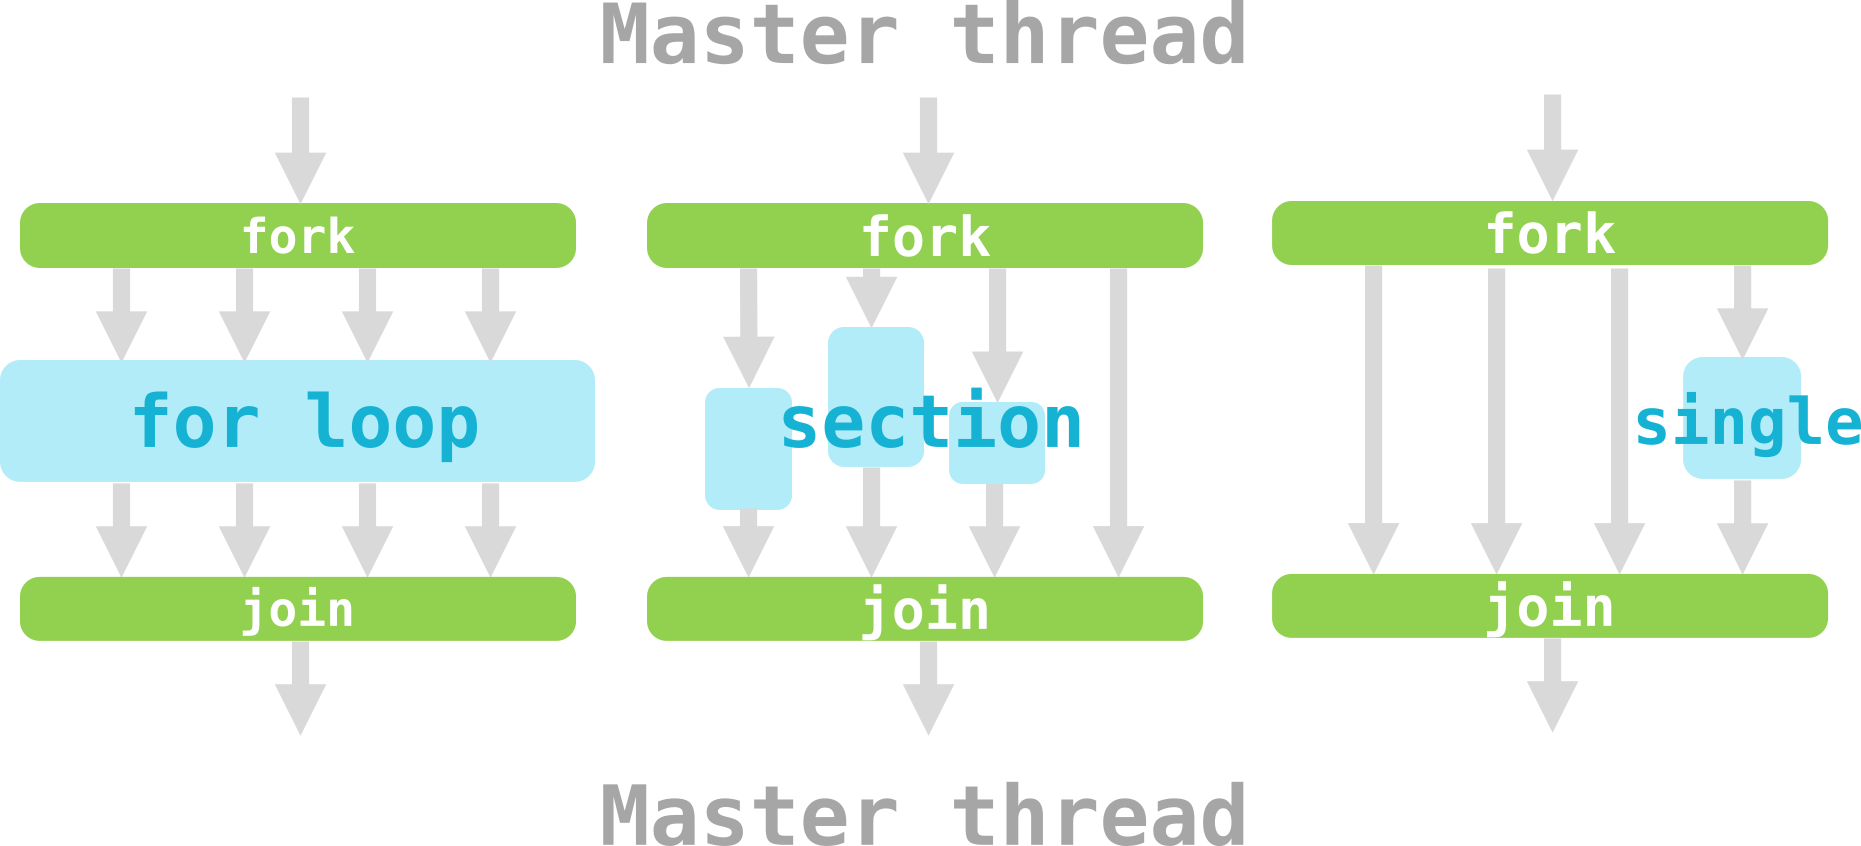
\includegraphics[width=1\linewidth]{day8_am/img/Work-distribution.png}
      \end{figure}
    \end{column}

    \begin{column}{0.3\textwidth}
      \vspace{2em}
      Work-distribution constructs:
      \begin{itemize}
        \item \textbf<1>{single}
        \item \textbf<2>{section}
        \item \textbf<3>{for}
      \end{itemize}
    \end{column}

  \end{columns}
\end{frame}

\begin{frame}[fragile]{\textit{parallel} Directive}
  \vspace{-10pt} % Align minted to the top
  \begin{minted}[fontsize=\small,highlightlines={5},highlightcolor=Khaki1]{c}
#include <stdio.h>
#include <omp.h>
int main() {
  printf("Welcome to OpenMP!\n");
  #pragma omp parallel
  {
    int ID = omp_get_thread_num();
    printf("hello(%d)", ID);
    printf("world(%d)\n", ID);
  }
  printf("Bye!");
  return 0;
}
      \end{minted}
\end{frame}

\begin{frame}[fragile]{Combined Constructs and Directives}
  \textbf{Example 2: \textit{parallel for} Directive}
  \begin{columns}[T] % align columns at top
    \begin{column}{0.5\textwidth}
      \vspace{-10pt} % Align minted to the top
      \begin{minted}[fontsize=\scriptsize]{c}
// Addition of two vectors
for (int i = 0; i < N; i++) {
    c[i] = a[i] + b[i];
}
      \end{minted}
    \end{column}

    \begin{column}{0.5\textwidth}
      \vspace{-10pt} % Align minted to the top
      \begin{minted}[fontsize=\scriptsize, highlightlines={2}]{c}
// Addition of two vectors
#pragma omp parallel for
for (int i = 0; i < N; i++) {
    c[i] = a[i] + b[i];
}
      \end{minted}
    \end{column}
  \end{columns}
  \begin{figure}
    \centering
    \includegraphics<1-2>[width=0.55\linewidth]{day8_am/img/parallel-for-1.png}
  \end{figure}
  \centering \uncover<2>{\emoji{exploding-head} Not 4x speed up}

  \uncover<3>{\emoji{hugging-face} \textbf{Overhead}: any combination of excess or indirect computation time, memory, bandwidth, or other resources that are required to perform a specific task.}
\end{frame}

\begin{frame}[fragile]{Loop Schedule}


  \begin{minted}[fontsize=\scriptsize]{c}
#pragma omp parallel for
for (int i = 0; i < N; i++) {
    c[i] = f(i); // What if f is not O(1)
}
\end{minted}

  Workload is unbalanced!

\end{frame}

\begin{frame}[fragile]{Loop Schedule}
  \begin{figure}
    \centering
    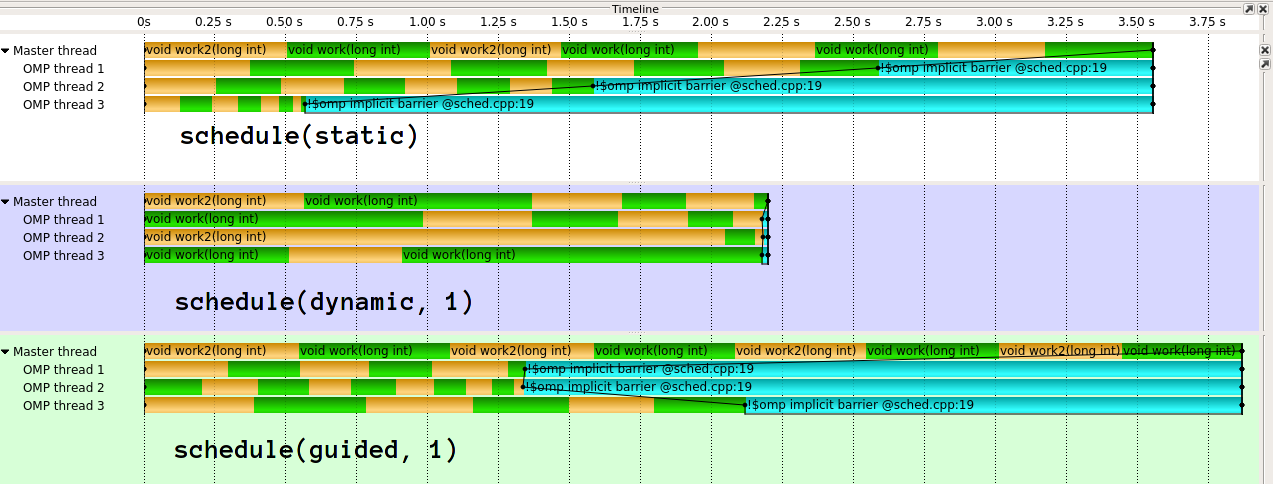
\includegraphics[width=0.8\linewidth]{day8_am/img/schedule-trace.png}
  \end{figure}

  \centering
  Static, Dynamic, Guided, Runtime, Auto

\end{frame}

\begin{frame}[fragile]{Loop Schedule - Static}

  \begin{minted}[fontsize=\scriptsize]{c}
#pragma omp parallel for schedule(static)
for (int i = 0; i < N; i++) {
    c[i] = f(i);
}
\end{minted}

  Static, Dynamic, Guided, Auto
\end{frame}

\begin{frame}[fragile]{Loop Schedule - Dynamic}

  \begin{minted}[fontsize=\scriptsize]{c}
#pragma omp parallel for schedule(dynamic, 2)
for (int i = 0; i < N; i++) {
    c[i] = f(i); // What is f is O(N^2)
}
\end{minted}

  \begin{itemize}
    \item[\emoji{thumbs-up}] Pros: More flexible scheduling
    \item[\emoji{thumbs-down}] Cons: More overhead in scheduling
  \end{itemize}

\end{frame}

\begin{frame}[fragile]{Nested \textit{for} Loop}
  \begin{columns}[T] % align columns at top
    \begin{column}{0.5\textwidth}
      \vspace{-10pt} % Align minted to the top
      \begin{minted}[fontsize=\scriptsize]{c}
// Matrix Element-wise Addition
#pragma omp parallel for
for (int i = 0; i < n; i++) {
    for (int j = 0; j < n; j++) {
        c[i][j] = a[i][j] + b[i][j];
    }
}
      \end{minted}
    \end{column}

    \begin{column}{0.5\textwidth}
      \vspace{-10pt} % Align minted to the top
      \begin{minted}[fontsize=\scriptsize, highlightlines={1}]{c}
#pragma omp parallel for collapse(2)
for (int i = 0; i < n; i++) {
    for (int j = 0; j < n; j++) {
        c[i][j] = a[i][j] + b[i][j];
    }
}
      \end{minted}
    \end{column}
  \end{columns}
\end{frame}
\subsection{Shared Data and Data Hazards}

\begin{frame}[fragile]{Example: Data Hazards in Summation}
\begin{minted}[fontsize=\scriptsize]{c}
#include <stdio.h>
#include "omp.h"
int main() {
    int a[100];
    int sum = 0;
    // initialize
    for (int i = 0; i < 100; i++) a[i] = i + 1;
    // Sum up from 1 to 100
#pragma omp parallel for
    for (int i = 0; i < 100; i++) {
        sum += a[i];
    }
    printf("Sum = %d\n", sum);
}
\end{minted}
\end{frame}

\begin{frame}[fragile]{How Data Hazards Happen?}
\begin{columns}[T]
    \begin{column}{0.7\textwidth}
        \begin{figure}
            \centering
            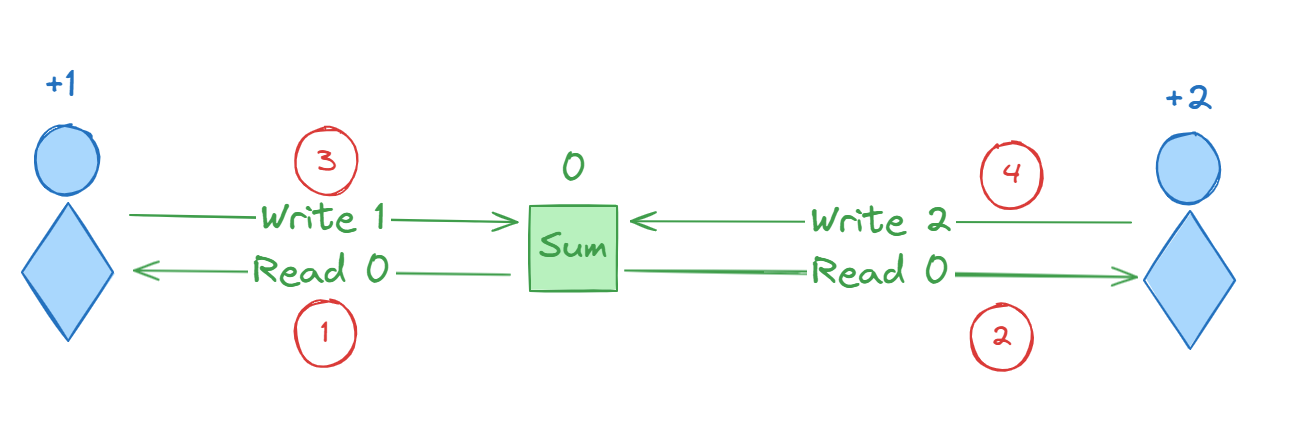
\includegraphics[width=\textwidth]{day8_am/img/hazard_illustration.png}
        \end{figure}
    \end{column}
    \begin{column}{0.3\textwidth}
        \begin{figure}
            \centering
            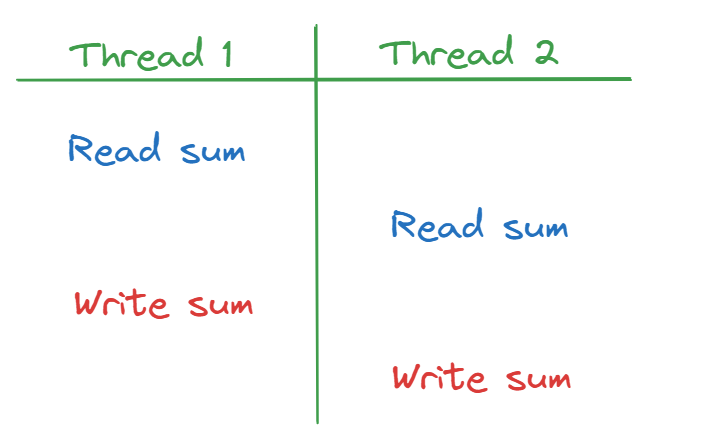
\includegraphics[width=\textwidth]{day8_am/img/hazard_schedule.png}
        \end{figure}
    \end{column}
\end{columns}
\end{frame}

\begin{frame}[fragile]{Scope and Data Hazard}
\begin{columns}[T]
    \begin{column}{0.5\textwidth}
        \begin{itemize}
            \item Shared \& private data in default
            \item Explicit scopes definition
            \begin{itemize}
                \item \textit{private}
                \item \textit{shared}
                \item \textit{firstprivate}
                \item \textit{lastprivate}
            \end{itemize}
            \item Data hazards happen when operating shared data
        \end{itemize}
    \end{column}
    \begin{column}{0.5\textwidth}
        \begin{minted}[fontsize=\scriptsize]{c}
    int sum = 0;
    // Sum up from 1 to 100
#pragma omp parallel for
    for (int i = 0; i <= 99; i++) {
        sum += a[i];
    }
\end{minted}
    \end{column}
\end{columns}
\end{frame}

\begin{frame}[fragile]{Resolve Data Hazard}
\begin{itemize}
    \item Critical Section
    \item Atomic Operations
    \item Reduction
\end{itemize}
\end{frame}

\begin{frame}[fragile]{Example: Solution with Critical Section}
\begin{columns}[T]
    \begin{column}{0.5\textwidth}
        \begin{itemize}
            \item Only one thread can enter critical section at the same time.
            \item A critical section can contain multiple statements.
        \end{itemize}
    \end{column}
    \begin{column}{0.5\textwidth}
\begin{minted}[fontsize=\scriptsize]{c}
#pragma omp parallel for
    for (int i = 0; i < 100; i++) {
#pragma omp critical
        { sum += a[i]; }
    }
    printf("Sum = %d\n", sum);
\end{minted}
    \end{column}
\end{columns}

\end{frame}

\begin{frame}[fragile]{Example: Solution with Atomic Operation}
\begin{columns}[T]
    \begin{column}{0.5\textwidth}
        \begin{itemize}
            \item Atomic operation cannot be separated.
            \item Only can be applied to one operation
            \item Limited set of operators supported
        \end{itemize}
    \end{column}
    \begin{column}{0.5\textwidth}
\begin{minted}[fontsize=\scriptsize]{c}
#pragma omp parallel for
    for (int i = 0; i < 100; i++) {
#pragma omp atomic
        sum += a[i];
    }
    printf("Sum = %d\n", sum);
\end{minted}
    \end{column}
\end{columns}
\end{frame}

\begin{frame}[fragile]{Example: Solution with Reduction}
\begin{columns}[T]
    \begin{column}{0.45\textwidth}
        \begin{itemize}
            \item Create temporary private variables for each thread
            \item Reduce these private variables in the end
            \item Limited set of operators supported
        \end{itemize}
    \end{column}
    \begin{column}{0.55\textwidth}
\begin{minted}[fontsize=\scriptsize]{c}
#pragma omp parallel for reduction(+:sum)
    for (int i = 0; i < 100; i++) {
        sum += a[i];
    }
    printf("Sum = %d\n", sum);
\end{minted}
    \end{column}
\end{columns}
\end{frame}

\begin{frame}[fragile]{Comparison}
\begin{itemize}
    \item Critical Region: Based on locking
    \item Atomic Operation: Based on hardware atomic operations
    \item Reduction: only synchronize in the end

\end{itemize}
\end{frame}

\begin{frame}[fragile]{Another Example: GEMM}
    \begin{minted}[fontsize=\scriptsize]{c}
    // General Matrix Multiplication (GEMM)
    for (int i = 0; i < N; i++) {
        for (int j = 0; j < N; j++) {
            c[i][j] = 0;
            for (int k = 0; k < N; k++) {
                c[i][j] += a[i][k] * b[k][j];
            }
        }
    }
    \end{minted}
\end{frame}

\begin{frame}[fragile]{Another Example: GEMM}
    \begin{minted}[fontsize=\scriptsize]{c}
#pragma omp parallel for collapse(3) reduction(+ : c)
    for (int i = 0; i < N; i++) {
        for (int j = 0; j < N; j++) {
            c[i][j] = 0;
            for (int k = 0; k < N; k++) {
                c[i][j] += a[i][k] * b[k][j];
            }
        }
    }
    \end{minted}
\end{frame}
\subsection{Miscellaneous}

\begin{frame}{OpenMPI}
\begin{columns}
    \begin{column}{.5 \textwidth}

    \textbf{\large Modular Component Architecture(MCA)}

    \begin{itemize}
        \item MCA framework
        \item MCA component
        \item MCA module
    \end{itemize}
            
    \end{column}

    \begin{column}{.5 \textwidth}
        \begin{figure}
            \centering
            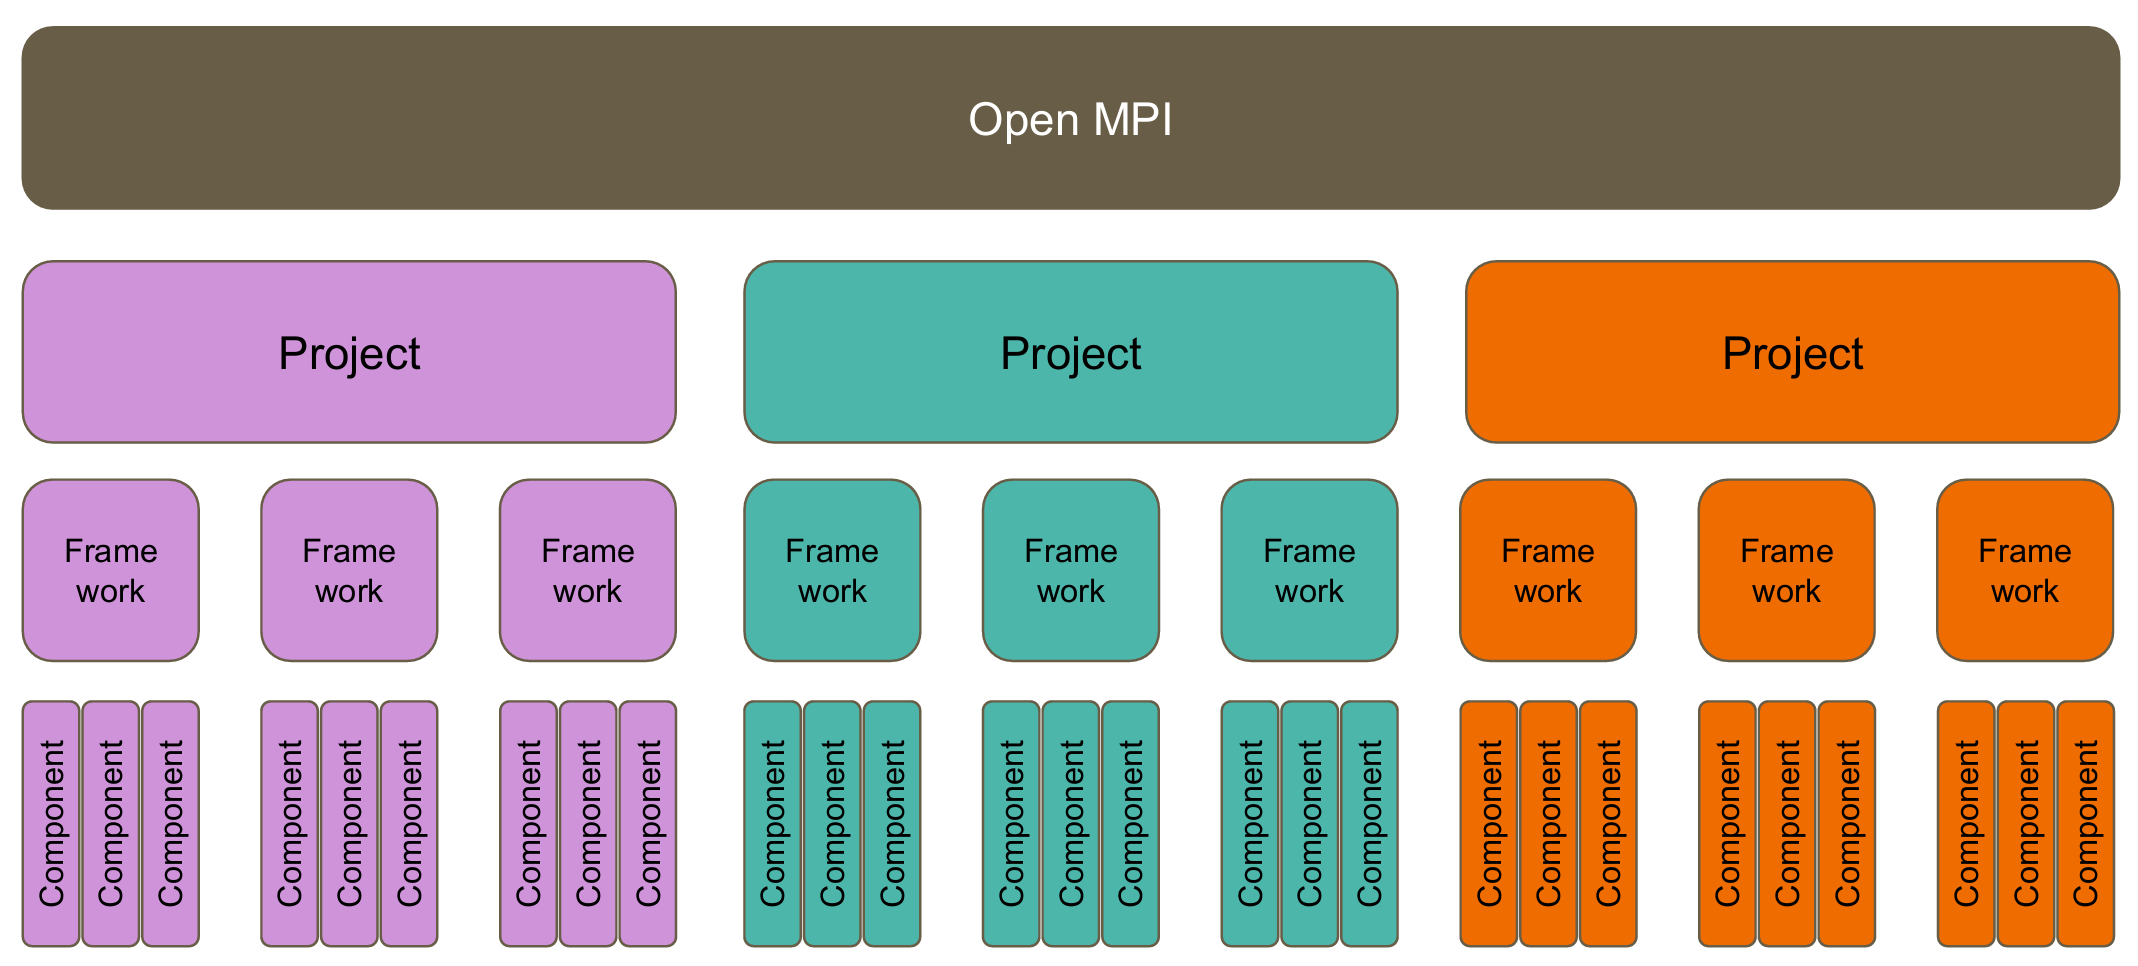
\includegraphics[width=1\linewidth]{day8_am/img/mpi/ompi_arch.png}
            \caption{OpenMPI Overall Architecture Terminology}
            \label{fig:ompi_arch}
        \end{figure}
    \end{column}    
\end{columns}
\end{frame}

\begin{frame}{OpenMPI}
\begin{columns}
    \begin{column}{.5 \textwidth}

    \textbf{\small 3 Types of OpenMPI Framework}

    \begin{itemize}
        \item In the MPI layer (OMPI)
        \item In the run-time layer (ORTE)
        \item In the operating system/platform layer (OPAL)
    \end{itemize}


    You might think of these frameworks as ways to group MCA parameters by function. (e.g. btl in OMPI)

    
    \end{column}

    \begin{column}{.5 \textwidth}
        \begin{figure}
            \centering
            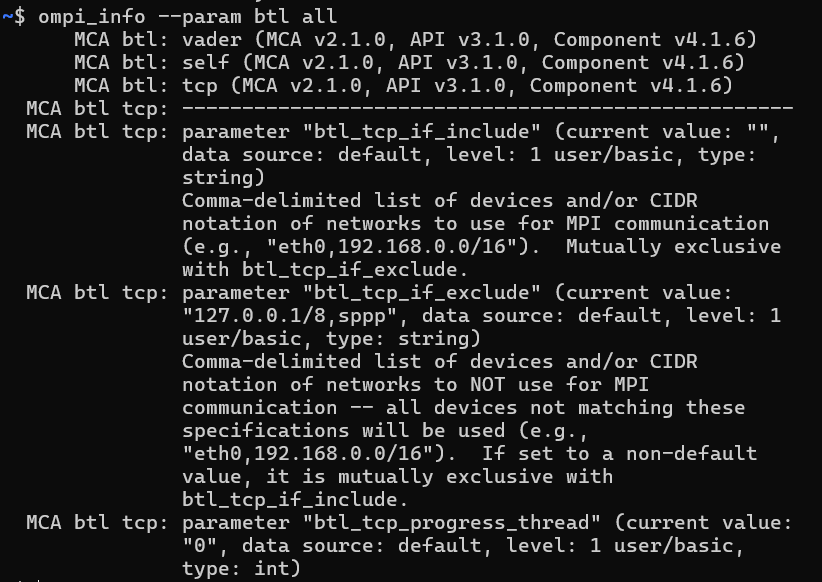
\includegraphics[width=1\linewidth]{day8_am/img/mpi/ompi_info.png}
            \caption{ompi\_info}
            \label{fig:ompi_info}
        \end{figure}
    \end{column}    
\end{columns}
\end{frame}

\begin{frame}[fragile]{OpenMPI(Installation) cont.}
\begin{columns}
    \begin{column}{.5 \textwidth}

    \textbf{\small Specify Compilers}
    
    {\scriptsize ./configure CC=/path/to/clang \\}

    {\scriptsize CXX=/path/to/clang++ FC=/path/to/gfortran ...}

    \vspace{1cm}
      \textbf{\small Static or Shared ?}
    {\scriptsize \begin{itemize}
        \item --enable-static / --disable-static (default)

        libmpi.a

        \item --enable-shared / --disable-shared

        libmpi.so
    \end{itemize}}
    \end{column}

    
    
    \begin{column}{.5 \textwidth}
        \textbf{\small Communication Library}
        
        UCX (Unified Communication X)

        {\scriptsize --with-ucx[=UCX\_INSTALL\_DIR]}
        
        \vspace{1cm}
        
        \textbf{\small With CUDA support}

        {\scriptsize ./configure --with-cuda[=/path/to/cuda]}
    \end{column}    
\end{columns}
\end{frame}

\begin{frame}[fragile]{OpenMPI (mpirun)}

\begin{itemize}
    \item -x [env]

    Passes environment variables to remote nodes.

    \item --bind-to core

    \item -hostfile [hostfile]

    \item ...
\end{itemize}
\end{frame}

% \begin{frame}{Loading MPI On Our Cluster}
% \begin{itemize}
%     \item \$ module load openmpi/5.0.3-pe46zvn
%     \item \$ module load intel-oneapi-mpi/2021.13.0-hpxfbao
% \end{itemize}
% \end{frame}

% \begin{frame}{Profiling and Tuning MPI Programs}
%     Later lectures. (7.12)
% \end{frame}

\section{MPI}

\begin{frame}{History}
    \begin{columns}
    
        \begin{column}{0.55\textwidth}

    \begin{itemize}
        \item \textbf{Before 1990's}: Many libraries. 

        Writing code was a \alert{\textbf{difficult}} task.

        \vspace{0.2cm}
        \hrule{}
        \vspace{0.2cm}
        {\textbf{Models commonly adopted: Message Passing Model}}
        
        An application \alert{\textbf{passes messages}} among processes in order to perform a task.

        e.g. Job assignment, Results of sub-problems...
        
    \end{itemize}
    \end{column}

        \begin{column}{0.45\textwidth}
            \begin{itemize}
                \item Supercomputing '92

                Defined a \alert{\textbf{standard interface}}

                \item 1994

                MPI-1

                \item 2025.6.5
            
                MPI-5.0 Standard Release
            \end{itemize}
        \end{column}
    \end{columns}
    %\footnotetext{https://mpitutorial.com/tutorials/mpi-introduction/}

    %\footnotetext{https://www.mpi-forum.org/docs/}
\end{frame}

\begin{frame}{What is MPI}
    MPI, a \alert{\textbf{M}}essage \alert{\textbf{P}}assaing \alert{\textbf{I}}nterface.

    There exists many implementations:
    \begin{itemize}
        \item OpenMPI
        \item Intel-MPI
        \item MPICH
        \item HMPI (Hyper-MPI)
        \item ......
    \end{itemize}

    \textbf{Kindly Reminder}: Please do not mess up MPI implementations with MPI standard.
\end{frame}


\begin{frame}{Installation}
    \begin{itemize}
        \item OpenMPI
        
            Lab0
        \item Intel-MPI: Included in \href{https://www.intel.cn/content/www/cn/zh/developer/tools/oneapi/toolkits.html}{Intel- neAPI}
        
            Can be installed using spack

        \item HMPI: \href{https://support.huawei.com/enterprise/zh/doc/EDOC1100228708/c5d7ef16}{Huawei}
    \end{itemize}
\end{frame}

\begin{frame}[fragile]{Hello MPI World!}
    \begin{minted}[fontsize=\scriptsize]{c}
#include <mpi.h>
#include <stdio.h>
int main(int argc, char** argv) {
    MPI_Init(&argc, &argv);
    int world_size;
    MPI_Comm_size(MPI_COMM_WORLD, &world_size);
    int world_rank;
    MPI_Comm_rank(MPI_COMM_WORLD, &world_rank);
    char processor_name[MPI_MAX_PROCESSOR_NAME];
    int name_len;
    MPI_Get_processor_name(processor_name, &name_len);
    printf("Hello world from processor %s, rank %d out of %d processors\n",
    processor_name, world_rank, world_size);
    MPI_Finalize();
    return 0;
}
    \end{minted}
\end{frame}

\subsection{Basic Concepts}

\begin{frame}{Communicator}
    \begin{block}{Definition}
        A communicator defines a group of processes that have the ability to communicate with one another.
        
        Each process has a \alert{\textbf{unique rank}}.
    \end{block}
\end{frame}


\begin{frame}{Communicator (cont.)}
\begin{columns}
    \begin{column}{.6\textwidth}
        \begin{itemize}
        \item MPI\_COMM\_WORLD
        \end{itemize}
        \begin{figure}
            \centering
            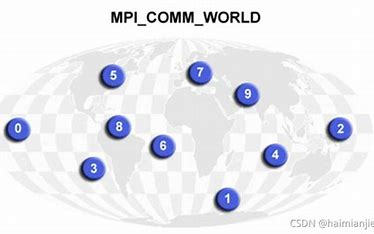
\includegraphics[width=\linewidth]{day8_am/img/mpi/mpi_comm_world.png}
            \caption{}
            \label{fig:mpi_comm_world}
        \end{figure}
    \end{column}
\end{columns}

\end{frame}


\begin{frame}{Communicator (cont.)}
\begin{columns}
    \begin{column}{.6\textwidth}
    \begin{itemize}
        \item MPI\_COMM\_SPLIT

        \begin{itemize}
            \item comm: The communicator that will be used as the basis for the new communicators.
            \item color: Which new communicator each processes will belong.
            \item key: The ordering (rank) within each new communicator.
            \item new\_comm: [OUT]
        \end{itemize}
    \end{itemize}
    \end{column}
        \begin{column}{.4\textwidth}
        \begin{figure}
            \centering
            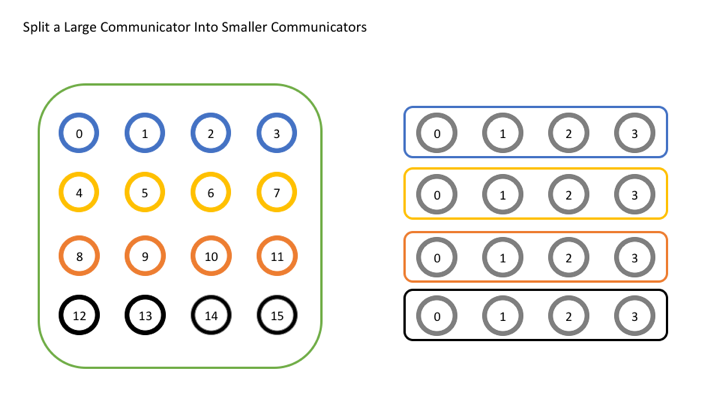
\includegraphics[width=1.0\linewidth]{day8_am/img/mpi/commsplit.png}
        \end{figure}
    \end{column}
\end{columns}

\end{frame}

\begin{frame}{Blocking vs Non-blocking}
    \begin{columns}
        \begin{column}{.5\textwidth}
            \textbf{\large Blocking}

            It does not return until the message data and envelope have been \alert{\textbf{safely stored away}} so that the sender is free to modify the send buffer. 
            
            The message might be copied directly into the \alert{\textbf{matching receive buffer}}, or it might be copied into a \alert{\textbf{temporary system buffer}}.
        \end{column}
        \begin{column}{.5\textwidth}
            \textbf{\large Non-blocking}

            A nonblocking call initiates the operation, but does not complete it. 
            
            They will return \alert{\textbf{almost immediately}}.
            
        \end{column}
    \end{columns}
\end{frame}

\begin{frame}{Order}
    \textbf{\large Messages are non-overtaking}
    
    Order is preserved.(Only under single thread)

If a sender sends two messages in succession to the same destination, and both match the same receive, then this operation cannot receive the second message if the first one is still pending. 

If a receiver posts two receives in succession, and both match the same message, then the second receive operation cannot be satisfied by this message, if the first one is still pending.
\end{frame}

\begin{frame}{Fairness}
    MPI makes \alert{\textbf{no guarantee}} of fairness in the handling of communication.

    There may be starvation.

    \begin{example}
        Rank1 $\rightarrow ^{send}$ Rank0

        Rank2 $\rightarrow^{send}$ Rank0

        Rank0 $\leftarrow^{receive}$ from any source.
    \end{example}
\end{frame}
\subsection{Point-to-Point Communication}

\begin{frame}[fragile]{Blocking Send and Receive}
\begin{columns}
    
\begin{column}{.42\textwidth}
\begin{tabular}{c}
      \begin{minted}[fontsize=\footnotesize]{c}
int MPI_Send(
    const void* buffer,
    int count,
    MPI_Datatype datatype,
    int recipient,
    int tag,
    MPI_Comm communicator);    
      \end{minted}
\end{tabular}
\end{column}

\begin{column}{.58\textwidth}
\textbf{\large Parameters:}

\begin{itemize}
    \item \textbf{buffer} The buffer to send.

    \item \textbf{count} The number of elements to send.

    \item \textbf{datatype} The type of one buffer element.

    \item \textbf{recipient} The rank of the recipient MPI process.

    \item \textbf{tag} The tag to assign to the message.

    \item \textbf{communicator} The communicator in which the standard send takes place.
\end{itemize}

\end{column}
\end{columns}
\end{frame}

\begin{frame}[fragile]{Blocking Send and Receive}
\begin{columns}
    
\begin{column}{.4\textwidth}
\begin{tabular}{c}
    \begin{minted}[fontsize=\footnotesize]{c}
int MPI_Recv(
    void* buffer,
    int count,
    MPI_Datatype datatype,
    int sender,
    int tag,
    MPI_Comm communicator,
    MPI_Status* status);
      \end{minted}
\end{tabular}
\end{column}

\begin{column}{.6\textwidth}
\textbf{\large Parameters:}
{\footnotesize
\begin{itemize}
    \item \textbf{buffer} The buffer to receive.

    \item \textbf{count} The number of elements to receive.

    \item \textbf{datatype} The type of one buffer element.

    \item \textbf{sender} The rank of the sender MPI process.

    \item \textbf{tag} The tag to assign to the message.

    \item \textbf{communicator} The communicator in which the standard receive takes place.

    \item \textbf{status} The variable in which store the status of the receive operation. Pass MPI\_STATUS\_IGNORE if unused.
\end{itemize}
}
\end{column}
\end{columns}
\end{frame}

\begin{frame}{MPI\_Status}
    MPI\_Status represents the status of a reception operation.

    At least 3 attributes: 
    \begin{itemize}
        \item MPI\_SOURCE
        \item MPI\_TAG
        \item MPI\_ERROR
    \end{itemize}

    There may be additional attributes that are implementation-specific.
\end{frame}

\begin{frame}{Message Envelope}
    In addition to the data part, messages carry information that can be used to distinguish messages and selectively receive them.
    \begin{itemize}
        \item source
        \item destination
        \item tag
        \item communicator
    \end{itemize}
\end{frame}


\begin{frame}{Communication Mode}
\only<1>{
    \begin{itemize}
        \item \textbf{Buffer Mode}
        
        Can be started whether or not a matching receive was posted.
        Completion does not depend on the occurrence of a matching receive.
        \item \textbf{Synchronous Mode}

        Can be started whether or not a matching receive was posted.

        The send will be completed successfully only if a matching receive is posted.

        \item \textbf{Ready Mode}

        May be started only if the matching receive is already posted.

        \item \textbf{Standard Mode}

        Depends.
        
    \end{itemize}
}

\only<2>{
\footnotesize

    \begin{table}[]
\begin{tabular}{lll}

\textbf{Communication mode} & \textbf{Start time}   & \textbf{Completion time}                         \\
\hline
Buffer mode        & Immediately                 & Message has gone to buffer              \\
\hline
Synchronous mode   & Immediately                 & Matching receive has posted \\
\hline
Ready mode         & Matching receive has posted & When the send buffer can be reused      \\
\hline
Standard mode      & Depends                     & Depends  \\                  \hline      

\end{tabular}


\end{table}
}
\end{frame}

\begin{frame}[fragile]{Communication mode: A common mistake}

    \textbf{Note}: MPI\_Ssend will \textbf{always wait until the receive has been posted} on the receiving end.
    \begin{minted}[fontsize=\footnotesize]{c}
// n = 2
MPI_Comm_rank(comm, &my_rank);
MPI_Ssend(sendbuf, count, MPI_INT, my_rank ^ 1, tag, comm);
MPI_Recv(recvbuf, count, MPI_INT, my_rank ^ 1, tag, comm, &status);
      \end{minted}

    \onslide<1->{\emoji{thinking} What will happen?}

    \onslide<2>{\emoji{exploding-head} Deadlock! Any solutions?}
\end{frame}

\begin{frame}[fragile]{Communication mode: Solution}
    \begin{tabular}{c}
      \begin{minted}[fontsize=\footnotesize]{c}
// n = 2
MPI_Comm_rank(comm, &my_rank);
if (my_rank == 0) {
    MPI_Ssend(sendbuf, count, MPI_INT, 1, tag, comm);
    MPI_Recv(recvbuf, count, MPI_INT, 1, tag, comm, &status);
} else if (my_rank == 1) {
    MPI_Recv(recvbuf, count, MPI_INT, 0, tag, comm, &status);
    MPI_Ssend(sendbuf, count, MPI_INT, 0, tag, comm);
}
      \end{minted}
    \end{tabular}

    \onslide<2->{\emoji{thinking} Any other solutions?}
\end{frame}

\begin{frame}[fragile]{Blocking Send and Receive}
\begin{columns}
    
\begin{column}{.5\textwidth}
\begin{minted}[fontsize=\footnotesize]{c}
int MPI_Sendrecv(
    const void* buffer_send,      
    int count_send,
    MPI_Datatype datatype_send,
    int recipient,
    int tag_send,
    void* buffer_recv,
    int count_recv,
    MPI_Datatype datatype_recv,
    int sender,
    int tag_recv,
    MPI_Comm communicator,
    MPI_Status* status);
\end{minted}
\end{column}

\begin{column}{.5\textwidth}
\begin{block}{Notice}
    The buffers used for send and receive must be different.
\end{block}

\onslide<2->{\emoji{thinking} Any other solutions?}

\end{column}
\end{columns}
\end{frame}

\begin{frame}[fragile]{Non-Blocking Send and Receive}
\begin{block}{Recall}
    A nonblocking call initiates the operation,
    but does not complete it.
    
    They will return almost immediately.
\end{block}
    
\begin{minted}[fontsize=\footnotesize]{c}
int MPI_Isend(const void* buffer,
              int count,
              MPI_Datatype datatype,
              int recipient,
              int tag,
              MPI_Comm communicator,
              MPI_Request* request);
\end{minted}
\end{frame}

\begin{frame}{Synchronization}
    \begin{columns}
        \begin{column}{.5\textwidth}
        
            \begin{itemize}
                \item \textbf{MPI\_Test}

                MPI\_TEST(request, flag, status)
                
                \begin{itemize}

                \item Checks if a non-blocking operation is complete at a given time.
                
                \item flag=true if completes.
                \end{itemize}
            \end{itemize}
        \end{column}

        \begin{column}{.5\textwidth}
            \begin{itemize}
                \item \textbf{MPI\_Wait}

                MPI\_WAIT(request, status)

                \begin{itemize}
                    \item Waits for a non-blocking operation to complete. 
                    \item That is, unlike MPI\_Test, MPI\_Wait will block until the underlying non-blocking operation completes.
                \end{itemize}
            \end{itemize}
        \end{column}
    \end{columns}
\end{frame}

\begin{frame}[fragile]{Non-Blocking Send and Receive(Deadlock revisit)}
\begin{minted}[fontsize=\footnotesize]{c}
MPI_Request req;
MPI_Isend(sendbuf, 0x100, MPI_INT, my_rank^1, 0, MPI_COMM_WORLD, &req);
MPI_Recv(recvbuf, 0x100, MPI_INT, my_rank^1, 0, MPI_COMM_WORLD, MPI_STATUS_IGNORE);
\end{minted}
\end{frame}
\subsection{Collective Communication}

\begin{frame}{Synchronization}
    \begin{columns}
        \begin{column}{.5\textwidth}
        
            \begin{itemize}
                \item \textbf{MPI\_Barrier}

                MPI\_Barrier(COMM)

                Blocks all MPI processes in the given communicator until they all call this routine.
            \end{itemize}
        \end{column}

        \begin{column}{.5\textwidth}
            \begin{figure}
                \centering
                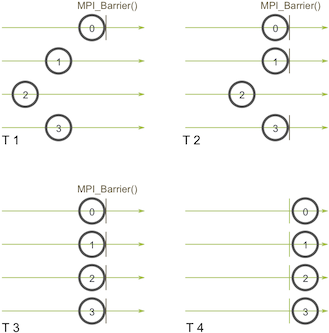
\includegraphics[width=0.7\linewidth]{day8_am/img/mpi/barrier.png}
                \caption{MPI\_Barrier}
                \label{fig:barrier}
            \end{figure}
        \end{column}
    \end{columns}
\end{frame}

\begin{frame}[fragile]{Broadcast: One to All}
    \begin{columns}
    
\begin{column}{.4\textwidth}
\begin{minted}[fontsize=\footnotesize]{c}
int MPI_Bcast(
    void* buffer,
    int count,
    MPI_Datatype datatype,
    int emitter_rank,
    MPI_Comm communicator);
\end{minted}

{\footnotesize
\begin{itemize}
    \item \textbf{emitter\_rank} 
The rank of the MPI process that broadcasts the data, all other processes receive the data broadcasted.
\end{itemize}
}
\end{column}

\begin{column}{.6\textwidth}
\begin{figure}
    \centering
    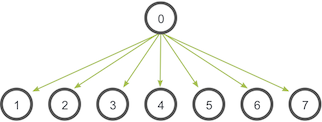
\includegraphics[width=0.75\linewidth]{day8_am/img/mpi/bcast.png}
    \caption{Bcast}
    \label{fig:bcast}
\end{figure}
\end{column}
\end{columns}
\end{frame}

\begin{frame}[fragile]{Broadcast: One to All}
\textbf{\large Why not Send and Receive?}

\begin{minted}[fontsize=\tiny]{c}
double start = MPI_Wtime();

if(my_rank == 0){
    for(int i=1; i<=31; i++)
        MPI_Send(sendbuf, 0x10000, MPI_INT, i, 0, MPI_COMM_WORLD);
}else{
    MPI_Recv(recvbuf, 0x10000, MPI_INT, 0, 0, MPI_COMM_WORLD, MPI_STATUS_IGNORE);
}

double end = MPI_Wtime();

if(my_rank == 0) printf("[Send Recv] Finished in %f seconds\n", my_rank, end-start);

start = MPI_Wtime();
MPI_Bcast(&sendbuf, 0x10000, MPI_INT, 0, MPI_COMM_WORLD);
end = MPI_Wtime();

if(my_rank == 0) printf("[Bcast] Finished in %f seconds\n", my_rank, end-start);
\end{minted}

\end{frame}

\begin{frame}{Broadcast: Tree based algorithm}
    \begin{figure}
        \centering
        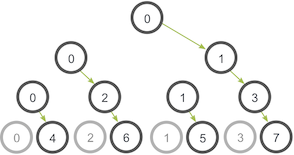
\includegraphics[width=0.65\linewidth]{day8_am/img/mpi/broadcasttree.png}
    \end{figure}
\end{frame}

\begin{frame}[fragile]{Scatter(One to All)}
    \begin{columns}
    
\begin{column}{.5\textwidth}
\begin{minted}[fontsize=\scriptsize]{c}
int MPI_Scatter(
    const void* buffer_send,
    int count_send,
    MPI_Datatype datatype_send,
    void* buffer_recv,
    int count_recv,
    MPI_Datatype datatype_recv,
    int root,
    MPI_Comm communicator);
\end{minted}

{\scriptsize
\begin{itemize}
    \item \textbf{count\_send}
    The number of elements to send to each process.

    \item \textbf{count\_receive}
    The number of elements in the receive buffer.
    
\end{itemize}
}
\end{column}

\begin{column}{.5\textwidth}
\begin{figure}
    \centering
    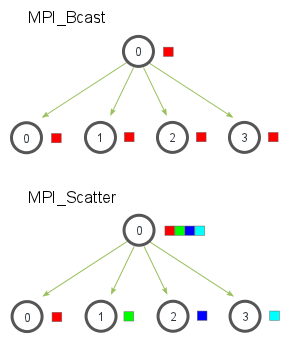
\includegraphics[width=0.8\linewidth]{day8_am/img/mpi/scatter.png}
    \caption{Scatter}
    \label{fig:scatter}
\end{figure}
\end{column}
\end{columns}
\end{frame}

\begin{frame}[fragile]{Gather: All to One}
    \begin{columns}
    
\begin{column}{.5\textwidth}
\begin{minted}[fontsize=\footnotesize]{c}
int MPI_Gather(
    const void* buffer_send,
    int count_send,
    MPI_Datatype datatype_send,
    void* buffer_recv,
    int count_recv,
    MPI_Datatype datatype_recv,
    int root,
    MPI_Comm communicator);
\end{minted}

\end{column}

\begin{column}{.5\textwidth}
\begin{figure}
    \centering
    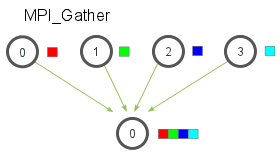
\includegraphics[width=0.75\linewidth]{day8_am/img/mpi/gather.png}
    \caption{MPI\_Gather}
\end{figure}
\end{column}
\end{columns}
\end{frame}

\begin{frame}[fragile]{Scatter and Gather}
    \begin{example}
        \textbf{Compute average}
    \end{example}
     \begin{minted}[fontsize=\scriptsize]{c}
MPI_Scatter(buffer, 0x1000000/4, MPI_DOUBLE, local_buffer, 0x1000000/4, MPI_DOUBLE, 0, MPI_COMM_WORLD);
double local_avg = 0;
for(int i=0; i<0x1000000/4; i++){
    local_avg += local_buffer[i];
}
local_avg /= 0x1000000/4;
double avgs[4];
MPI_Gather(&local_avg, 1, MPI_DOUBLE, avgs, 1, MPI_DOUBLE, 0, MPI_COMM_WORLD);
\end{minted}
\end{frame}

\begin{frame}[fragile]{Allgather(All to All)}
    \begin{columns}
    
\begin{column}{.5\textwidth}
\begin{minted}[fontsize=\footnotesize]{c}
int MPI_Allgather(
    const void* buffer_send,
    int count_send,
    MPI_Datatype datatype_send,
    void* buffer_recv,
    int count_recv,
    MPI_Datatype datatype_recv,
    MPI_Comm communicator);
\end{minted}

Actually MPI\_Gather + MPI\_Bcast.

\end{column}

\begin{column}{.5\textwidth}
\begin{figure}
    \centering
    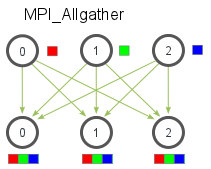
\includegraphics[width=0.75\linewidth]{day8_am/img/mpi/allgather.png}
    \caption{MPI\_Allgather}
    \label{fig:enter-label}
\end{figure}
\end{column}
\end{columns}
\end{frame}

\begin{frame}[fragile]{Reduce}
    \begin{columns}
    
\begin{column}{.5\textwidth}
\begin{minted}[fontsize=\footnotesize]{c}
int MPI_Reduce(
    const void* send_buffer,
    void* receive_buffer,
    int count,
    MPI_Datatype datatype,
    MPI_Op operation,
    int root,
    MPI_Comm communicator);
\end{minted}

\end{column}

\begin{column}{.5\textwidth}
\begin{figure}
    \centering
    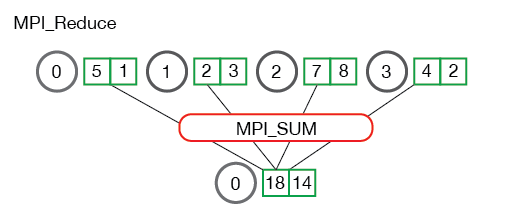
\includegraphics[width=0.75\linewidth]{day8_am/img/mpi/reduce.png}
    \caption{Reduce}
    \label{fig:reduce}
\end{figure}
\end{column}
\end{columns}
\end{frame}

\begin{frame}[fragile]{Reduce}
    \begin{example}
        \textbf{Compute average revisit}
    \end{example}
     \begin{minted}[fontsize=\scriptsize]{c}
MPI_Scatter(buffer, 0x1000000/4, MPI_DOUBLE, local_buffer, 0x1000000/4, MPI_DOUBLE, 0, MPI_COMM_WORLD);
double local_avg = 0;
for(int i=0; i<0x1000000/4; i++){
    local_avg += local_buffer[i];
}
local_avg /= 0x1000000/4;
double global_avg;
MPI_Reduce(&local_avg, &global_avg, 1, MPI_DOUBLE, MPI_SUM, 0, MPI_COMM_WORLD);
\end{minted}
\end{frame}
\subsection{Example}

\begin{frame}{Task}
\begin{columns}
    
\begin{column}{0.5\textwidth}

\scriptsize
    Implement a data validation algorithm using SHA512.
    
    Algorithm procedure:
    \begin{enumerate}
        \item Tile the input file into blocks of 1MB. (If the last block is smaller than 1MB, pad it with zeros.)
        \item For the $i^{th}$ block, concatenate it with the validation sum SHA512 of $(i-1)^{th}$ block and calculate validation sum of SHA512.
        \item The validation sum of the last block is considered as the validation sum of the entire file.
    \end{enumerate}

    \textbf{Source}: HPC Game 2024
\end{column}

\begin{column}{0.5\textwidth}
    \begin{figure}
        \centering
        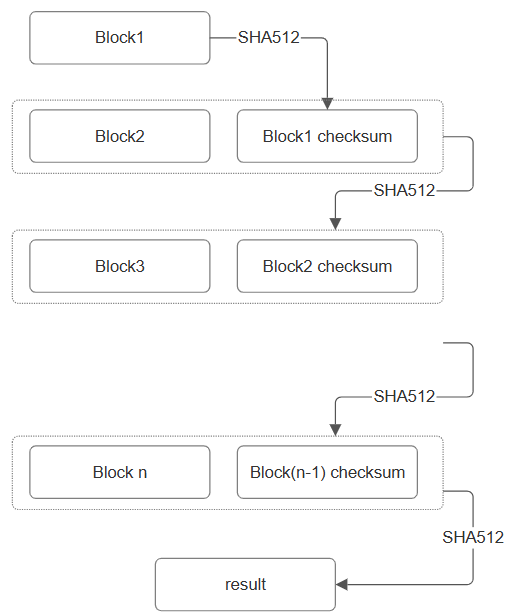
\includegraphics[width=0.65\linewidth]{day8_am/img/mpi/SHA512.png}
    \end{figure}
\end{column}
\end{columns}
\end{frame}

\begin{frame}[fragile]{Baseline Code}
    \begin{columns}
    \begin{column}{.5\textwidth}
\begin{minted}[fontsize=\tiny]{c}
int num_block = (len + BLOCK_SIZE - 1) / BLOCK_SIZE;
uint8_t prev_md[SHA512_DIGEST_LENGTH];

EVP_MD_CTX *ctx = EVP_MD_CTX_new();
EVP_MD *sha512 = EVP_MD_fetch(nullptr, "SHA512", nullptr);

SHA512(nullptr, 0, prev_md);
\end{minted}
        \end{column}
        
        \begin{column}{.5\textwidth}
        \begin{minted}[fontsize=\tiny]{c}
for (int i = 0; i < num_block; i++) {
    uint8_t buffer[BLOCK_SIZE]{};
    EVP_DigestInit_ex(ctx, sha512, nullptr);
    std::memcpy(buffer, data + i * BLOCK_SIZE,
                std::min(BLOCK_SIZE, len - i * BLOCK_SIZE));
    EVP_DigestUpdate(ctx, buffer, BLOCK_SIZE);
    EVP_DigestUpdate(ctx, prev_md, SHA512_DIGEST_LENGTH);

    unsigned int len = 0;
    EVP_DigestFinal_ex(ctx, prev_md, &len);
}
              \end{minted}
        
        \begin{block}{\scriptsize Notice}
        \scriptsize
            EVP\_DigestUpdate(a);
            EVP\_DigestUpdate(b);
            
            Equivalent to EVP\_DigestUpdate(concate(a,b)) !
        \end{block}
        \end{column}

    \end{columns}
    
\end{frame}

\begin{frame}{Analysis}
    Computation is dependent on the result of the previous one.
    
    How to exploit MPI?

\end{frame}

\begin{frame}{Analysis}
    Computation is dependent on the result of the previous one.
    
    How to exploit MPI?

    \vspace{1cm}

    \textbf{Answer:}
    
    File \textbf{I/O} accounts! We can \textbf{overlap} I/O operations with computation.
\end{frame}

\begin{frame}[fragile]{MPI Code}
    \begin{columns}
    \begin{column}{.5\textwidth}
        \textbf{\scriptsize Non-Blocking receives the previous block's checksum.}
            \begin{minted}[fontsize=\tiny]{c}
if(i != 0) {
  MPI_Irecv((void *)prev_md,
          SHA512_DIGEST_LENGTH,
          MPI_UINT8_T,
          sender,
          0,
          MPI_COMM_WORLD,
          &request);
}
              \end{minted}
        \end{column}
        
        \begin{column}{.5\textwidth}
        \textbf{\scriptsize Meanwhile... File I/O and Digest}
                \begin{minted}[fontsize=\tiny]{c}
istrm.seekg(i * BLOCK_SIZE);
istrm.read(reinterpret_cast<char *>(data + i * BLOCK_SIZE), std::min(BLOCK_SIZE*local_size, file_size - i * BLOCK_SIZE));

for(int j=i; j<upper_bound; j++){
    uint8_t buffer2[BLOCK_SIZE]{};
    EVP_DigestInit_ex(ctx[j-i], sha512, nullptr);
    std::memcpy(buffer2, data + j * BLOCK_SIZE,
                std::min(BLOCK_SIZE, len - j * BLOCK_SIZE));
    EVP_DigestUpdate(ctx[j-i], buffer2, BLOCK_SIZE);
}

if(i != 0){
    MPI_Wait(&request, MPI_STATUS_IGNORE);
}
              \end{minted}
        \end{column}
        
    \end{columns}
    
\end{frame}

\begin{frame}[fragile]{MPI Code (cont.)}
    \begin{columns}
    \begin{column}{.45\textwidth}
        \textbf{\scriptsize Non-blocking send my checksum}
        \begin{minted}[fontsize=\tiny]{c}
unsigned int len = 0;
for(int j=i; j<upper_bound; j++){
    EVP_DigestUpdate(ctx[j-i], prev_md, SHA512_DIGEST_LENGTH);
    EVP_DigestFinal_ex(ctx[j-i], prev_md, &len);
}
if(upper_bound != num_block) {
    MPI_Isend(prev_md,
        SHA512_DIGEST_LENGTH,
        MPI_UINT8_T,
        recepient,
        0,
        MPI_COMM_WORLD,
        &request);
}
              \end{minted}
        \end{column}
        
        \begin{column}{.55\textwidth}
        \begin{figure}
            \centering
            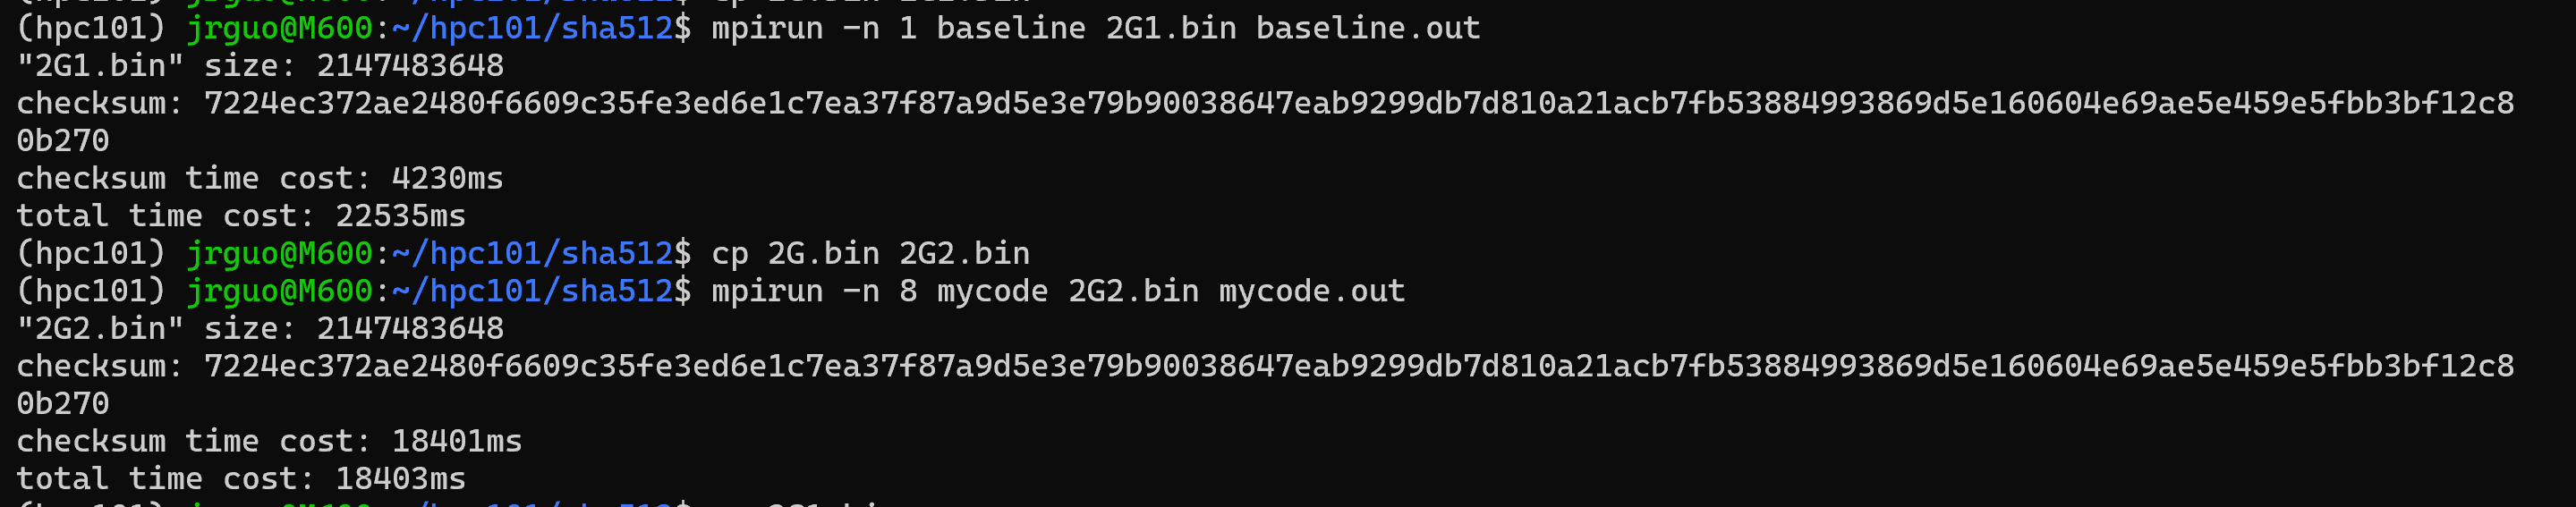
\includegraphics[width=1.0\linewidth]{day8_am/img/mpi/speedup.png}
        \end{figure}

        \vspace{0.5cm}

        \end{column}
        
    \end{columns}
    
\end{frame}

\begin{frame}{Wrap up}
    \begin{figure}
            \centering
            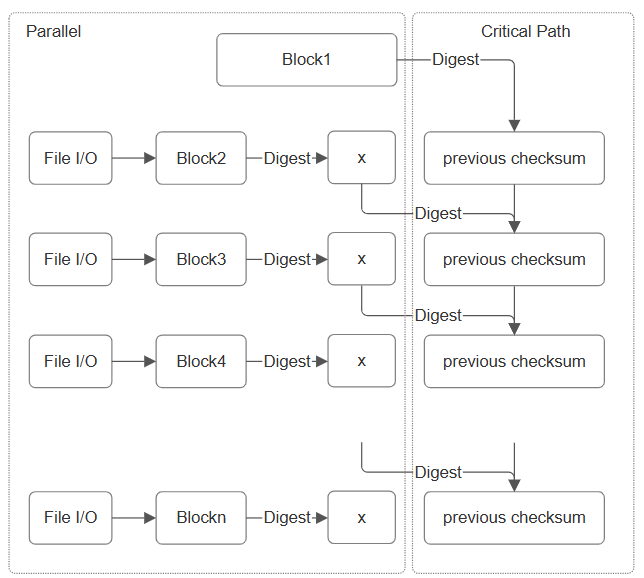
\includegraphics[width=0.45\linewidth]{day8_am/img/mpi/SHA512para.png}
    \end{figure}
\end{frame}

\subsection{Miscellaneous}

\begin{frame}{OpenMPI}
\begin{columns}
    \begin{column}{.5 \textwidth}

    \textbf{\large Modular Component Architecture(MCA)}

    \begin{itemize}
        \item MCA framework
        \item MCA component
        \item MCA module
    \end{itemize}
            
    \end{column}

    \begin{column}{.5 \textwidth}
        \begin{figure}
            \centering
            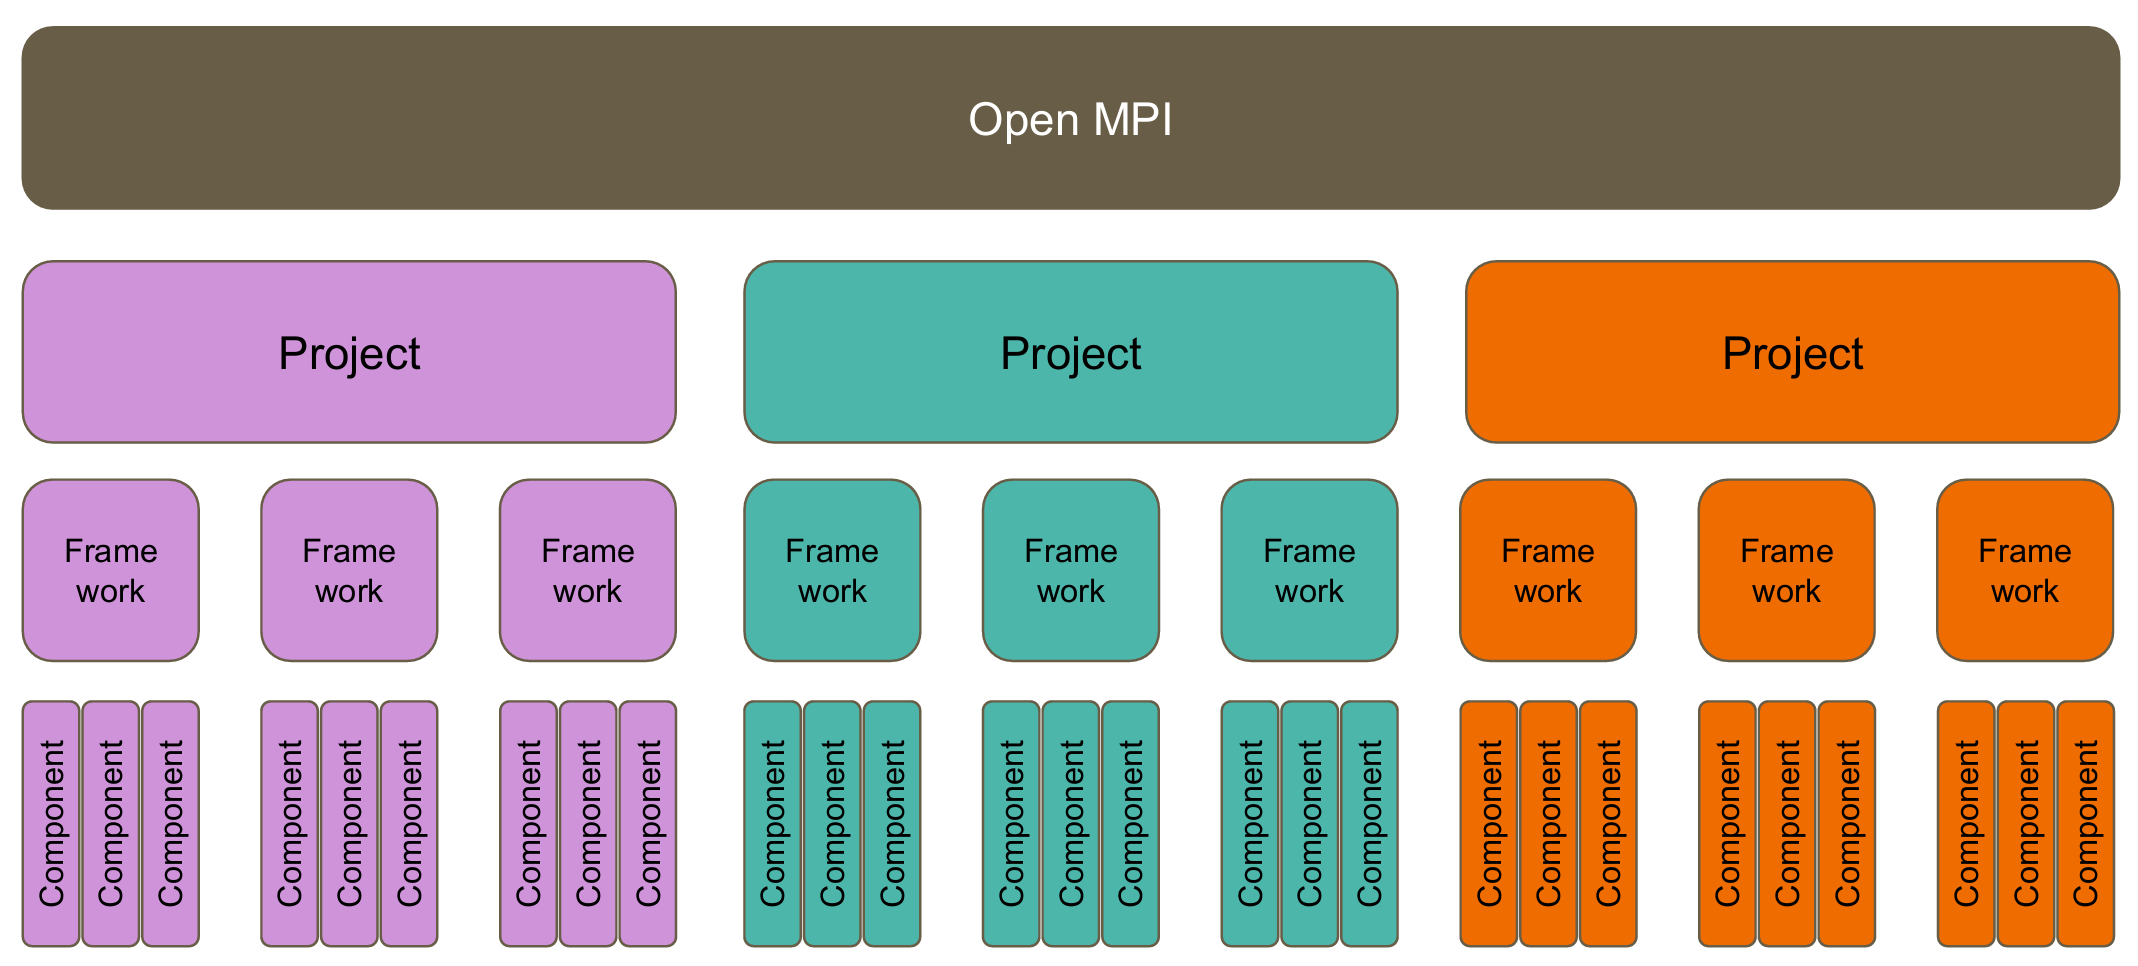
\includegraphics[width=1\linewidth]{day8_am/img/mpi/ompi_arch.png}
            \caption{OpenMPI Overall Architecture Terminology}
            \label{fig:ompi_arch}
        \end{figure}
    \end{column}    
\end{columns}
\end{frame}

\begin{frame}{OpenMPI}
\begin{columns}
    \begin{column}{.5 \textwidth}

    \textbf{\small 3 Types of OpenMPI Framework}

    \begin{itemize}
        \item In the MPI layer (OMPI)
        \item In the run-time layer (ORTE)
        \item In the operating system/platform layer (OPAL)
    \end{itemize}


    You might think of these frameworks as ways to group MCA parameters by function. (e.g. btl in OMPI)

    
    \end{column}

    \begin{column}{.5 \textwidth}
        \begin{figure}
            \centering
            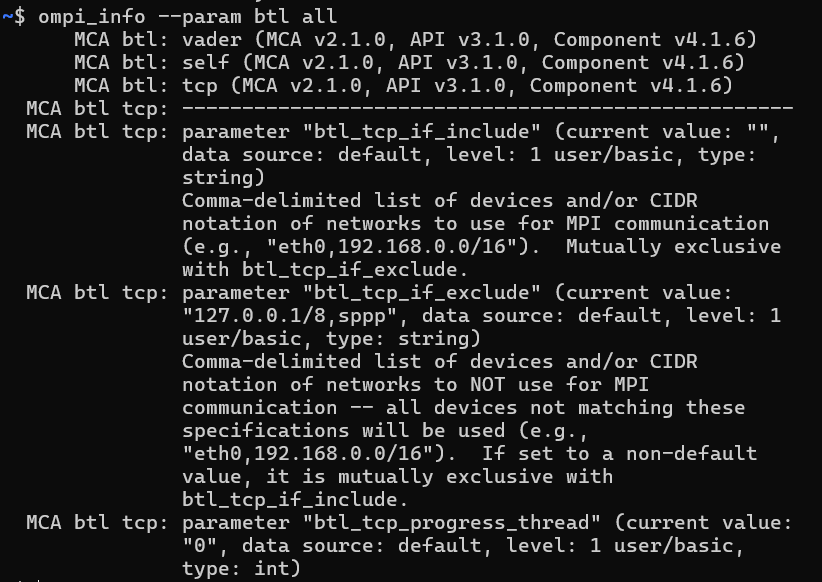
\includegraphics[width=1\linewidth]{day8_am/img/mpi/ompi_info.png}
            \caption{ompi\_info}
            \label{fig:ompi_info}
        \end{figure}
    \end{column}    
\end{columns}
\end{frame}

\begin{frame}[fragile]{OpenMPI(Installation) cont.}
\begin{columns}
    \begin{column}{.5 \textwidth}

    \textbf{\small Specify Compilers}
    
    {\scriptsize ./configure CC=/path/to/clang \\}

    {\scriptsize CXX=/path/to/clang++ FC=/path/to/gfortran ...}

    \vspace{1cm}
      \textbf{\small Static or Shared ?}
    {\scriptsize \begin{itemize}
        \item --enable-static / --disable-static (default)

        libmpi.a

        \item --enable-shared / --disable-shared

        libmpi.so
    \end{itemize}}
    \end{column}

    
    
    \begin{column}{.5 \textwidth}
        \textbf{\small Communication Library}
        
        UCX (Unified Communication X)

        {\scriptsize --with-ucx[=UCX\_INSTALL\_DIR]}
        
        \vspace{1cm}
        
        \textbf{\small With CUDA support}

        {\scriptsize ./configure --with-cuda[=/path/to/cuda]}
    \end{column}    
\end{columns}
\end{frame}

\begin{frame}[fragile]{OpenMPI (mpirun)}

\begin{itemize}
    \item -x [env]

    Passes environment variables to remote nodes.

    \item --bind-to core

    \item -hostfile [hostfile]

    \item ...
\end{itemize}
\end{frame}

% \begin{frame}{Loading MPI On Our Cluster}
% \begin{itemize}
%     \item \$ module load openmpi/5.0.3-pe46zvn
%     \item \$ module load intel-oneapi-mpi/2021.13.0-hpxfbao
% \end{itemize}
% \end{frame}

% \begin{frame}{Profiling and Tuning MPI Programs}
%     Later lectures. (7.12)
% \end{frame}

% Q&A
\begin{frame}[standout]
    \Huge\textsc{Thank You}
    \vfill
    \LARGE\textsc{Any Questions?}
\end{frame}

\end{document}